\section{System Design}
\label{sec:design}
AgentWorkShop is designed for industrial tasks whose agents, production
contexts, interfaces, and process signals vary between deployments. Its
architecture organizes these variations around shared task and operation
services, checks each proposed operation against the active production
context before device routing, and retains route-specific evidence that
distinguishes a command receipt from a measured process response.

\begin{figure*}[!t]
\centering
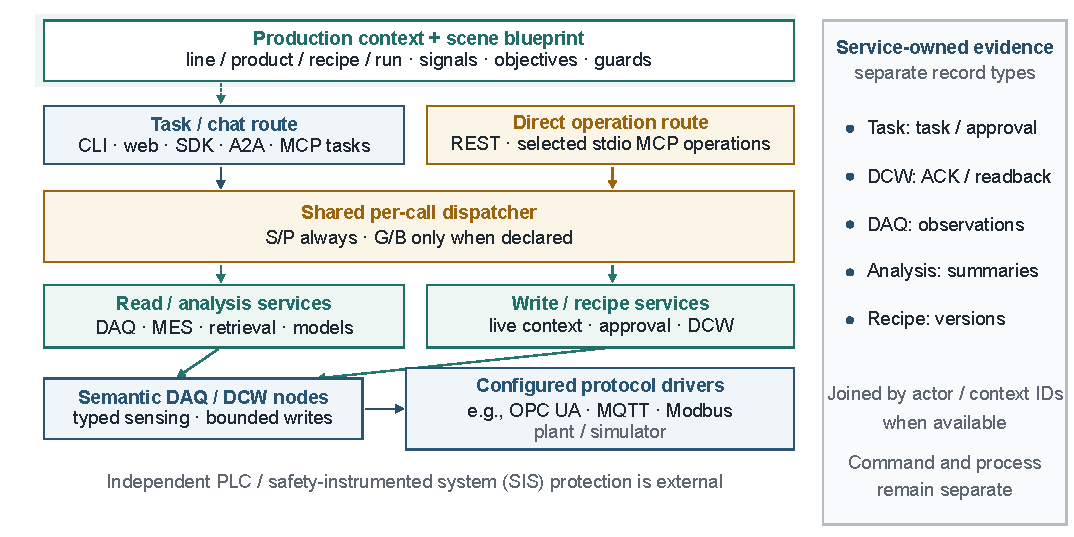
\includegraphics[width=\textwidth]{resources/fig-architecture-2026-9pt.pdf}
\caption{Architecture and record ownership. Task/chat routes enter the
collaboration runtime; direct REST and stdio-MCP calls enter shared dispatch
checks without creating a task. One dashed link marks configuration. Write
routes add approval and interval admission; recipe dispatch omits the
previous-recipe window. The shared dispatcher always
checks scope and channel policy, with grant and resource-binding checks applied
when required by the operation. Owning services retain distinct records; plant
controllers and safety systems retain equipment interlocks.}
\label{fig:arch}
\end{figure*}

\subsection{Design Rationale and Requirements}
\label{sec:principles}
Five requirements---scene variability, harness variability, operation
authority, outcome observability, and extensibility---shape the design.
Scene variability is represented by blueprints and semantic driver mappings;
harness variability by registered adapters; operation authority by shared
dispatch checks and route-specific guards and admission; outcome observability
by service-owned task, receipt, and observation records; and extensibility by
registered interfaces for agent engines and device drivers. Tool visibility
is separate from write authorization, and actuator writes converge on the
shared DCW admission point.

A scene blueprint bundles the process preset, signal inventory, DAQ/DCW driver
mappings, and target and guard rules; judged operation records and later
observations remain distinct evidence.

During setup, the integrator binds a validated blueprint to the active
line--product--recipe--run tuple, maps semantic nodes to drivers, and declares
target bands and guards. At runtime, the dispatcher checks current authority
before the handler issues a command; the handler returns a receipt, and DAQ
records subsequent observations.

\subsection{Layered Architecture}
\label{sec:layers}
\label{sec:arch}
Fig.~\ref{fig:arch} summarizes the access routes, shared dispatch path,
production services, semantic I/O, configured drivers, and service ownership
of records. Task and chat routes enter the
collaboration band, which contains workspaces, channels, task queues, shared
memory, mailboxes, task templates, and harness adapters. A \emph{task route}
is an execution path through this runtime; a \emph{harness adapter} connects
an agent engine to its task execution interface. Direct REST tool
calls and the stdio MCP operation bridge bypass task execution in that band
(the upper-right direct-operation entry in
Fig.~\ref{fig:arch}) and enter the shared governance block without creating a
task or starting a harness turn; MCP management and task methods remain on
their service routes. Direct calls resolve current route state at invocation,
without an agent-turn prompt or a task record.
The governance block projects the operation catalog and applies the per-call
checks; write routes add the approval card and the admission interval. The
context block supplies the active line--product--recipe--run tuple to the gate
and scene maps, objectives, and guards to the handlers. The dashed link from
that block in Fig.~\ref{fig:arch} marks this configuration relationship; the
runtime assembles prompt-time context from the same records. The service band,
behind a route-handler interface that selects an adapter, provides
acquisition, write control, analysis, retrieval, and optional model services.
Field I/O resolves semantic nodes to built-in or plugin drivers for a plant or
simulator.

Each band has a distinct responsibility: task/chat routes enter the runtime,
direct operations enter the dispatcher, and both use shared checks. Harness
adapters supply agent-specific interaction, semantic nodes hide protocol
details, and the driver registry provides the device-facing extension point.
Owning services retain task, command, observation, and version records
separately and link them to actor and production context.

\subsection{Cross-Module Execution Flow}
\label{sec:executionflow}
Fig.~\ref{fig:runtime} summarizes a task turn from entry through operation
execution, with route-specific evidence retained by owning services. Registered
harness adapters receive a scoped tool catalog during setup and supported
registry refreshes; the runtime assembles prompt-time production context from
current records for each agent turn. For each returned tool call, the shared dispatcher rechecks
invocation scope and channel policy and, for industrial operations, current
grant and binding conditions before handler selection. The selected handler
then applies route-specific guards, active-run checks, approval
revalidation, and device-I/O steps as applicable. Command receipts and later
process observations remain distinct records.

For an industrial operation $u$ by agent $a$ in channel $c$, define the
shared dispatch condition as
\begin{equation}
\mathcal{A}(a,c,u)=\bigwedge_{X\in\mathcal{C}(u)}X(a,c,u),
\label{eq:dispatch-contract}
\end{equation}
where $S$, $P$, $G$, and $B$ denote invocation scope, current channel policy,
runtime grant, and the agent's binding to referenced resources, respectively.
$\mathcal{C}(u)\subseteq\{S,P,G,B\}$ is the set of predicates declared for
operation $u$; it always contains $S$ and $P$. The grant predicate $G$ is
omitted only for an explicitly grant-exempt industrial tool, and $B$ is
included when the operation declares resource references. A declared
no-reference operation omits $B$. Each included check must pass before
handler selection. The policy predicate includes channel tool selection,
profile, and duty-separation checks where configured. Once these predicates
pass, the selected route applies its guards and approval, then rechecks
authority, context, and applicable limits before device dispatch.

For direct REST invocation, the service establishes $a$ and $c$ before applying
these checks: an agent token must match the requested agent identifier, or an
authenticated user must be the channel owner or an administrator. The manager
loads the channel-agent record and rechecks scope and policy; industrial
operations then pass the shared grant and binding checks. Handlers resolve live
production state from request identifiers and owning services.

Fig.~\ref{fig:execution} gives reference pseudocode summarizing the
registered-harness task path. Direct REST tool invocation
bypasses the task runtime and harness but enters the same shared dispatcher.
Route-specific timing, approval, and evidence rules are detailed in
Section~\ref{sec:modules}.

\begin{figure*}[!t]
\centering
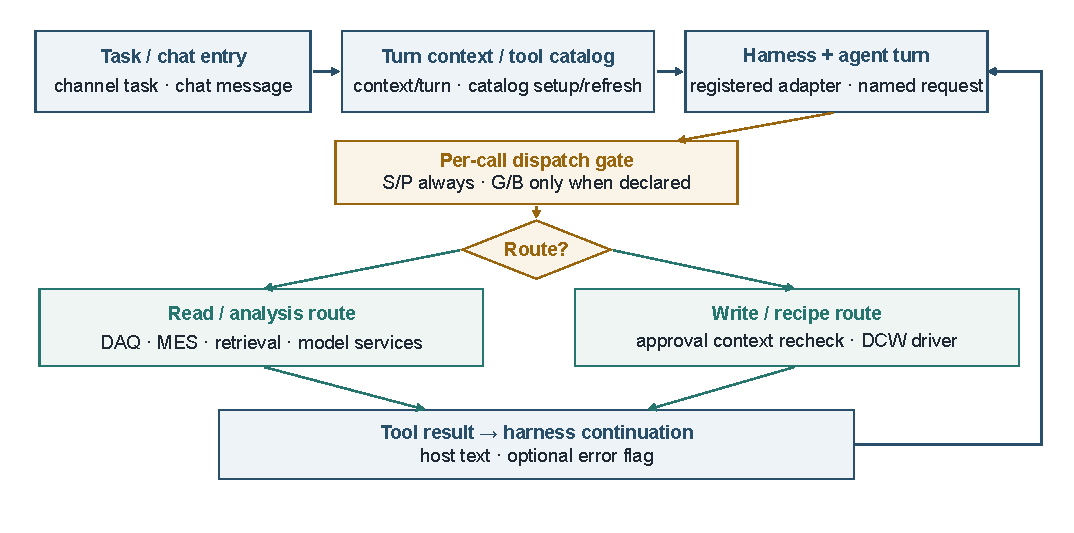
\includegraphics[width=\textwidth]{resources/fig-runtime-2026-9pt.pdf}
\caption{Registered-harness task flow. The runtime invokes the adapter with a
scoped catalog. Scope and channel policy are checked for every call; grant
applies to non-exempt industrial operations, and binding applies when resource
references are declared (figure label: S/P always, G/B only when declared). Failed
checks return tool errors. The read path
retrieves data. The write path applies route guards, approval and context
revalidation, DCW admission, and receipt grading; a later process observation
is separate. Results return to the harness. Device-level interlocks remain
with the configured plant-control layer.}
\label{fig:runtime}
\end{figure*}

\begin{figure}[!t]
\centering
\begin{algorithmic}[1]
\Require task $q$, channel $c$, bound agent $a$, registered scoped catalog $T$
\Ensure task result; any retained evidence remains with its owning service
\State $x_t \gets \Call{ResolvePromptContext}{c,q}$
\State $m \gets \Call{RetrieveMemory}{q}$
\State $p \gets \Call{AssemblePrompt}{q,x_t,m}$
\State $h \gets \Call{InvokeRegisteredHarness}{a,p,T}$
\ForAll{tool request $u$ returned by $h$}
  \State $g \gets \Call{CheckScopeAndChannelPolicy}{a,c,u}$
  \If{\textbf{not} $g$}
    \State \Call{EmitToolErrorToHarness}{h,u}; \textbf{continue}
  \EndIf
  \If{$u$ is an industrial operation}
    \State $v \gets \Call{CheckApplicableGrantBinding}{a,u}$
    \If{\textbf{not} $v$}
      \State \Call{EmitToolErrorToHarness}{h,u}
      \State \textbf{continue}
    \EndIf
  \EndIf
  \State $k \gets \Call{SelectHandler}{u}$
  \State $r \gets \Call{ExecuteRouteHandler}{k,a,c,u}$
  \Comment{handler resolves live state and may persist route-specific records}
  \State \Call{EmitDeclaredToolResultToHarness}{h,r}
\EndFor
\State \Return task state and tool results
\end{algorithmic}
\caption{Reference pseudocode for the registered-harness task path. Direct
operation calls use the shared dispatcher from their own entry point. Each
route persists its records through the owning service and returns its declared
response to the harness.}
\label{fig:execution}
\end{figure}
